\subsubsection{Point Mutation}
\label{sec:keen:gp:op:mutation:point}

    In GP, the capability to mutate program trees is paramount for infusing genetic diversity within a population. Among 
    various mutation operators, Point Mutation stands out. Its specialty lies in introducing delicate perturbations to a 
    program's structure, all the while upholding its syntactic and semantic consistency.

    \begin{definition}[Point Mutation]
        The \textit{point mutation} operator intricately selects a random node from a program tree, then searches for 
        another node boasting the same arity (i.e., number of child nodes). The initial node is subsequently replaced by 
        the latter, thus producing a variation of the original program while preserving the overarching tree structure.

        Mathematically, the operation can be delineated as:

        \begin{equation}
        M_{point}: \mathbb{P} \times [0,\, 1] \times [0,\, 1] \to \mathbb{P};\;
        (P,\, \mu_\textbf{c},\, \mu_\textbf{g}) \mapsto M_{point}(P,\, \mu_\textbf{c},\, \mu_\textbf{g})
        \end{equation}

        Explicating the parameters:

        \begin{itemize}
        \item \(P\): Represents a population of program trees.
        \item \(\mu_\textbf{c}\): Denotes the probability of a chromosome experiencing mutation.
        \item \(\mu_\textbf{g}\): Signifies the likelihood of a gene's selection for mutation.
        \end{itemize}
    \end{definition}

    The \textit{Keen} framework houses a lucid implementation of the Point Mutation operator, encapsulated in a succinct 
    four-step methodology:

    \begin{code}{
        Exemplification of Point Mutation in \textit{Keen}
    }{label=lst:keen:gp:op:mutation:point}{kotlin}
        val original = random node from program tree
        val replacements = nodes with identical arity as original
        val replacement = random node from replacements
        val mutated = program tree substituting original with replacement
    \end{code}

    The Point Mutation's cornerstone, especially in \textit{Keen}, is its knack for retaining the architectural 
    coherence of program trees amidst the introduction of genetic variations.

    \begin{remark}
        The emphasis on matching arity during node replacement is non-trivial. This meticulous approach ensures the 
        resultant mutated tree mirrors the structure of its predecessor. Such precision mitigates potential runtime 
        anomalies or semantic ambiguities, both of which could impede the evolutionary trajectory.
    \end{remark}

    While Point Mutation might seem simplistic at a cursory glance, its potency 
    shouldn't be underestimated. Its strategy of fine-tuned alterations forms a 
    judicious equilibrium between retaining the essence of high-performing 
    solutions and embarking on novel exploratory ventures.

    A visual representation of the Point Mutation operator's workings can be 
    observed in \vref{fig:keen:gp:op:mutation:point}.

    \begin{figure}[ht!]
        \centering
        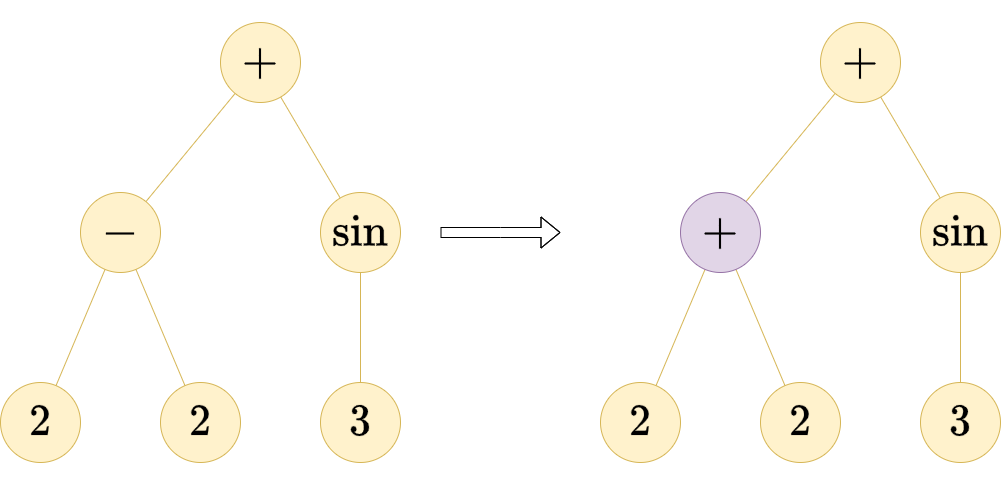
\includegraphics[width=0.5\textwidth]{img/keen/Point mutation.png}
        \caption{
        A graphical elucidation of the Point Mutation operator's effect on a 
        program tree. A random node is selected and substituted with another of 
        identical arity, resulting in a structurally-consistent variant of the 
        original tree.
        }
        \label{fig:keen:gp:op:mutation:point}
    \end{figure}
